The background chapter serves the purpose of providing a theoretical overview of the techniques applied to deal with the proposal of improving users' ability to operate a myoelectric prosthesis by training the user with the novel approach of confidence score feedback. The chapter will cover the usual applied methods of pattern recognition based myoelectric prosthesis control. The idea behind myoelectric prosthetic control is to  convert muscles signals (EMG signals), recorded from a user when performing a muscle contraction, into a movement performed by a prosthesis. The EMG signals are used to train a control system in recognizing a pattern in the EMG signals from different muscle contractions. The control system then decides which movement the prosthesis should perform, based on which pattern in the EMG signals that is recognized. The focus of this project is to investigate users' ability to adapt to how the control system wants the user to perform a muscle contraction for the desired movement to be performed by the prosthesis. The different processes of myoelectric prosthetic control the background chapter will cover are: the mechanics of the movements the control system will be trained to recognize, the generation of EMG signals, data acquisition, data processing, feature extraction, classification and control output. The pipeline of this process can be seen in \figref{fig:prothesis_control_pipeline}. Furthermore, the chapter will cover theory on how confidence scores are calculated, how user training has been used in previous studies and how real-time prosthesis control is evaluated.
%and how the results obtained from the prosthesis control evaluation are compared.

\begin{figure}[H] 
	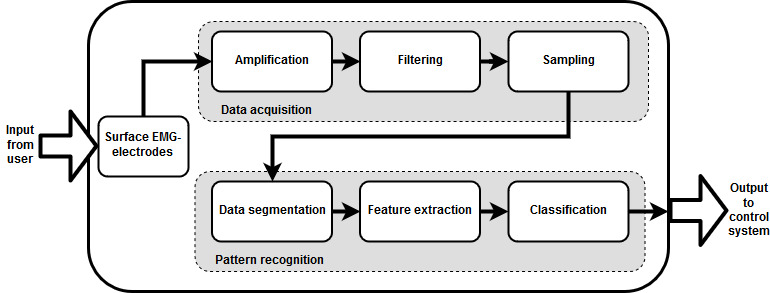
\includegraphics[width=0.9\textwidth]{figures/xBackground/prosthesis_control_pipeline}
	\caption{The figure shows the pipeline for myoelectric prosthetic control. The EMG signal from the user is first detected by the surface electrodes, after which it is amplified and filtered before it is sampled to process it digitally. To produce a control output the signal is subsequently segmented in windows from which features are extracted that are used to classify which movement has been made, and thus which movement should be performed by the prosthesis. The pipeline is adapted from \cite{Peerdeman2011}}
	\label{fig:prothesis_control_pipeline}
\end{figure}